\documentclass[conference]{./IEEEtran}

\usepackage{ulem} 
\usepackage{subfigure}
\usepackage{comment}
\usepackage{graphicx}
\usepackage{algorithm}
\floatname{algorithm}{Procedure}
\usepackage{multirow}
\usepackage{makeidx}
\usepackage{amsmath}
\usepackage{amssymb}
\usepackage{epsf}
\usepackage{pstricks}
\usepackage{pst-grad}
\usepackage{placeins}
\usepackage{url}
\usepackage{epsfig}
\usepackage{multirow}
\usepackage{pifont}
\usepackage{graphics}
\usepackage{color}
\usepackage{epsf}
\usepackage{mathcomp}
\usepackage{colordvi}
\usepackage{epsfig}
\usepackage{fancyhdr}
\usepackage{wasysym}
\usepackage{longtable}
\usepackage{afterpage}
\usepackage{colordvi}
\usepackage{latexsym}
\usepackage{float}
\usepackage{alphalph}
\usepackage{epic,eepic}
\usepackage{authblk}
\usepackage{algpseudocode}
\usepackage{mathptmx}
\usepackage{epstopdf}

\algnewcommand{\LineComment}[1]{\State \(\triangleright\) #1}


\newtheorem{definition}{Definition}
\newtheorem{example}{Example}
\newtheorem{note}{Note}
\newtheorem{operation}{Operation}
\newtheorem{axion}{Axion}
\newtheorem{remark}{Remark}
\newtheorem{lemma}{Lemma}
\newtheorem{theorem}{Theorem}

\ifCLASSINFOpdf
  % \usepackage[pdftex]{graphicx}
  % declare the path(s) where your graphic files are
  % \graphicspath{{../pdf/}{../jpeg/}}
  % and their extensions so you won't have to specify these with
  % every instance of \includegraphics
  % \DeclareGraphicsExtensions{.pdf,.jpeg,.png}
\else
  % or other class option (dvipsone, dvipdf, if not using dvips). graphicx
  % will default to the driver specified in the system graphics.cfg if no
  % driver is specified.
  % \usepackage[dvips]{graphicx}
  % declare the path(s) where your graphic files are
  % \graphicspath{{../eps/}}
  % and their extensions so you won't have to specify these with
  % every instance of \includegraphics
  % \DeclareGraphicsExtensions{.eps}
\fi

\hyphenation{op-tical net-works semi-conduc-tor}
\begin{document}

\title{Adaptive Display Scheme over Real-time Multimedia Communication on Mobile Devices}

%for single author (just remove % characters)
%%\date{}
%% \special{papersize=8.5in,11in}
%% \setlength{\pdfpageheight}{\paperheight}
%% \setlength{\pdfpagewidth}{\paperwidth}

%% \conferenceinfo{Submission to SoCC '14}{October, 2014, Seattle, WA, USA} 
%% \copyrightyear{2014} 
%% \copyrightdata{978-1-nnnn-nnnn-n/yy/mm} 
%% \doi{nnnnnnn.nnnnnnn}


%% \author{
%%   \IEEEauthorblockN{Mengbai Xiao}
%%   \IEEEauthorblockA{
%%     mxiao3@gmu.edu\\
%%     Department of Computer Science\\
%%     George Mason University}
%%     \and
%%   \IEEEauthorblockN{Songqing Chen}
%%   \IEEEauthorblockA{
%%     sqchen@gmu.edu\\ check the email\\
%%     Department of Computer Science\\
%%     George Mason University}
%% }



\maketitle

%\thispagestyle{empty}

%\sloppy
%------------------------------------------------------------------------------

\begin{abstract}
  Power saving is a significant issue at the mobile platform. Various
  techniques were proposed to extend the playback time of the
  videos. Backlight scaling is one of them and target the display
  subsystem. However, the multimedia content need to be delivered in a
  timely manner in the real-time communication. This raises challenges
  towards the existing backlight scaling technique. The backlight
  scaling technique is composed of computation intensive tasks,
  including the luminance histogram generation and the pixels
  luminance compensation on every frame. Multiple streaming sources in
  the video conference make this problem more difficult. Moreover,
  global luminance information is necessary for finding the optimal
  backlight levels across the streaming. This is clearly impossible in
  the real-time case. In this paper, we propose a greedy algorithm
  determining the backlight level of current frame only from the last
  one. We also take advantage of the GPU to relive the burden of the
  CPU on compensating the luminance of pixels. We integrate our
  prototype in the AppRTC, an Android app based on WebRTC, and find
  that our scheme can save up to 39.8\% energy during one
  communication session.
\end{abstract}


\section{Introduction}

As an advanced functionality, video call becomes an essential
component in many *communication applications/wechat, skype... check
in twin cloud paper*. The needs for unifying the interface is
increasingly desirable. The success of DATH *add name* hints people
the importance of HTTP in video/audio streaming scenarios. WebRTC as a
new API existing in HTML5 drops in developer's sight. Mainstream
browsers integrates the function into there production, i.e. Chrome,
Opera, Firefox. Developers can easily include video call in their page
via few lines of javascript code.

As the mobile market emerging, 




\section{Background}
\label{sec:background}
In this section, we briefly introduce the backlight scaling and WebRTC
for real-time video calls.

\subsection{Backlight scaling}
A visible image on a LCD display is produced by both backlight and the LCD
panel, which stores pixel color imformation. The perceptual luminance
is actually the backlight intensity compensated by the pixels. The
backlight scaling is a technique  exploiting
this characteristic. 
{\bf do we have another figure? captured from playing other videos? If
we do, can replace. But can delay till the last minute.}
Figure~\ref{fig:backlightscaling} sketches the high-level idea. As
shown in the figure, the energy for displaying the image can be
reduced by dimming the backlight. If  nothing else is done, 
 it will lead
to a darker version of this image. This distortion can be compensated
by concurrently increasing the luminance component of each pixel in
this image~\cite{PMLDV03, CHP07, CCS06, CSC02}. And increasing the
pixel brightness does not increase the power consumption of the
display.


\begin{figure}[!htb]
  \begin{center}
    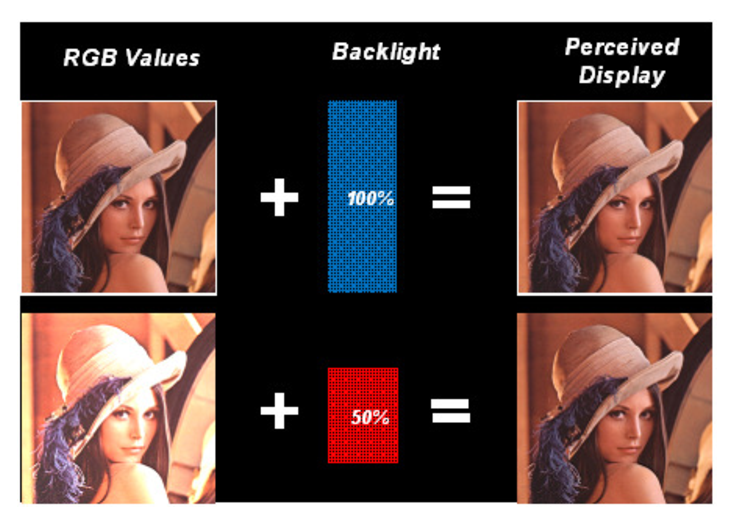
\includegraphics[scale=.75]{./figures/backlightscaling.eps}
    \caption{Backlight Scaling on LCD screen}
    \label{fig:backlightscaling}
  \end{center}
\end{figure}

However, directly applying backlight scaling to video playback faces
several challenges. Both extracting and enhancing the pixels luminance
component frame by frame demand processing a mass of data, and is
computation intensive.  For this reason, deploying these tasks during
the playback on the same CPU~\cite{CHP07, CSC02} is not practical
because of two reasons.  On the one hand, the CPU may not have enough
time to perform these computation intensive tasks without degrading
the video quality (e.g., frames per second or FPS) of the video playback. On
the other hand, the achieved power saving by dimming the backlight can be
offset by the power consumption due to these extra CPU operations. Hsiu et al. and Lin et
al.~\cite{LHH14, HLH11} proposed to skip the pixel compensation stage
and use a critical backlight level for each frame to avoid distorting
the image too badly. Ruggiero et al. suggested to offload the
luminance adjustment tasks to the hardware image processing unit (IPU)
integrated in Freescale’s multimedia application
processor~\cite{RBB08}. It exploits in a smart and efficient way to
implement a hardware assisted image compensation.
%% {\bf is this processor on the same machine or
%%   different machine?} 
Pasricha et al.~\cite{PMLDV03} and Cheng et al.~\cite{CMEDV07}
suggested to compute the backlight scaling data on a proxy server and
substitute the original video with a luminance-adjusted version. In
short, existing schemes (1) only target video-on-demand where the
video frame information is available in advance so that the computing
can be done before the playback, and (2) demand additional
infrastructure support for compensation or do not consider quality
degradation due to backlight dimming. So far, no scheme has been
considered for real-time video calls.

Compared to video-on-demand, real-time video calls are live streaming,
where each frame is produced on the fly and highly
delay-sensitive. Furthermore, video calls often invovle
multiple participants, and thus multiple frames from different sources
needed to be combined in real-time, leaving little computing power for
other tasks, such as pixel luminance compensation.

\subsection{Video Calls and WebRTC}

Video calls/conferecing are gaining increasing popularity.  On mobile
devices, many applications, such as Skype, QQ, and
Facetime~\cite{skype, qq, facetime}, {\bf this is not proper. add
  reference to each separately} all support video
calls/conferecing. The communication protocol of these applications is
proprietary to commercial companies, which precludes the communication
between different applications.  The increasing varities of mobile
devices, such as smartphones, tablets and emerging wearable devices,
make the situation even more complicated. To solve this fragmentation
problem in the real-time multimedia communication and also to provide
a cross-platform solution, Web Real-Time Communication
(WebRTC)~\cite{webrtcstandard} is proposed to enable video
communications via web browsers and standardized by the W3C and
IETF. Nowadays, mainstream browsers, e.g., Chrome, Firefox, Opera, all have integrated the WebRTC. The WebRTC
component~\cite{webrtcproject} implemented in the Chrome provides the
Javascript-style APIs. WebRTC can be linked to the native mobile apps
as an external libary.  WebRTC is now widely used by mobile
users. {\bf do you have some data about usage to put here? with
  references.} {\bf revise this later} However, given its video
streaming nature, the power consumption of video communication is
high, which has slowed down its pervasion.



%%% old 
%% \section{background}
%% \label{sec:background}

%% \subsection{Backlight scaling}
%% A visible image on LCD display is produced by both backlight and LCD
%% panel, which stores pixels color imformation. The perceptual luminance
%% is actually the backlight intensity compensated by the pixels. The
%% backlight scaling is a dedicated technique for LCD screen exploiting
%% this characteristics. This technique can be clearly illustrated in the
%% figure~\ref{fig:backlightscaling}. The energy of displaying one
%% picture can only be reduced by dimming the backlight, though it leads
%% to a darker version of this image. This distortion can be compensated
%% by concurrently increasing the luminance component of each pixel in
%% this image~\cite{PMLDV03, CHP07, CCS06, CSC02}. Fortunately, the
%% pixels brightness is uncorrelated to the power consumption of the
%% display.


%% \begin{figure}[!htb]
%%   \begin{center}
%%     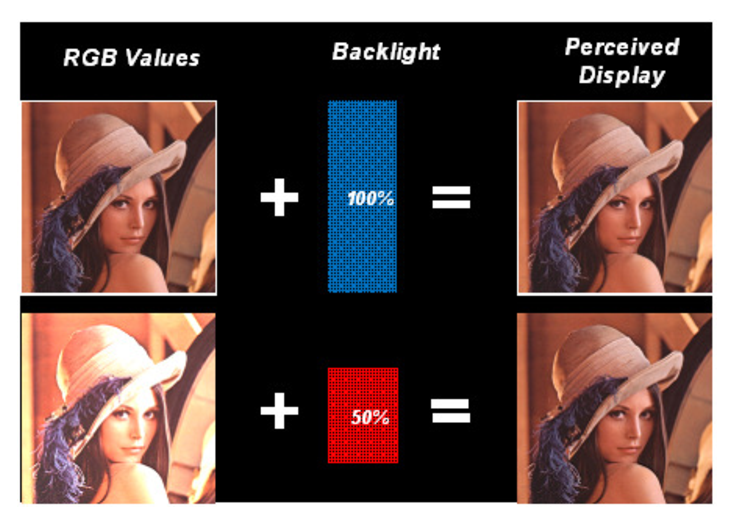
\includegraphics[scale=.75]{./figures/backlightscaling.eps}
%%     \caption{Backlight Scaling on LCD screen}
%%     \label{fig:backlightscaling}
%%   \end{center}
%% \end{figure}

%% Applying this technique in the video playbacks raises several
%% challenges. Both extracting and enhancing the pixels luminance
%% component frame by frame are the operations of processing a mass of
%% data. For this reason, deploying these tasks on the CPU~\cite{CHP07,
%%   CSC02} is not practical. On the one hand, the CPU may don't have
%% enough time to do these computation intensive tasks without degrading
%% the frames per second (FPS) of the video. On the other hand, the
%% achieved power savings by dimming backlight might be offset by these
%% extra operations. Hsiu et al. and Lin et al. ~\cite{LHH14, HLH11} proposed to
%% skip the pixels compensation stage and use a critical backlight level
%% of each frame to avoid distorting the image too badly. Ruggiero et
%% al. offload the luminance adjustment tasks to an independent
%% processor~\cite{RBB08}. Pasricha et al.~\cite{PMLDV03} and Cheng et
%% al.~\cite{CMEDV07} suggested to compute the backlight scaling data on
%% a proxy server and substitute the original video with a
%% luminance-adjusted version.


%% \subsection{WebRTC}

%% The conversational RTC protocols are the company proprietaries,
%% precluding the communication between different services.  The
%% prosperity of mobile devices, including smartphones, tablet
%% and emerging wearable devices, makes the situation more
%% complicated. To solve the fragmentation problem in the real-time
%% multimedia communication and also to provide a cross-platform
%% solution, Web Real-Time Communication (WebRTC)~\cite{webrtcstandard}
%% is proposed and standardized by the W3C and IETF. Nowadays, mainstream
%% browsers, e.g. Chrome, Firefox, Opera and etc., all have integrated
%% the WebRTC inside them. Not only does the WebRTC
%% component~\cite{webrtcproject} implemented in the Chrome provide the
%% Javascript-style APIs, but also it can be linked to the native mobile
%% apps as an external libary. In this paper, we build our prototype
%% based on the AppRTC, which is the Android version app incorperating
%% the WebRTC library.


\section{System Design}
\subsection{Backlight Scaling Algorithms}
The basic idea of luminance compensation is when the backlight is
dimmed, the luminance of frame pixels are enhanced. Thence the power
savings are achieved while no observable distortion exists. In next
sections, we denote the $t = 1, 2, ...$ as the frame index in a live
streaming. And the $Y_{t}^{max} \in [0, 255]$ is the max luminance of
frame $t$. The $b_{t} \in [0, 1]$ stands for the target backlight
level when the $t$th frame is rendering.

\subsubsection{Dynamic Programming}
Although the ideal case is the pixels of the $t$th frame are enhanced by
$(255 - Y_{t}^{max})$, so that the $b_{t}$ can be scaled to
$\frac{Y_{t}^{max}}{255}$, which is the minimum possible value, 
without losing any observable fidelity. However, if we do this
practically, two negative phenomenons are found:
\begin{itemize}
  \item{The {\it flickering} is found as the screen backlight varies
    dramatically.}
  \item{On devices, The backlight scale can't react in real-time
    manner. The hardware response the scaling directive in a short
    delay.}
\end{itemize}
Both of the facts should be taken into account when we scale the
backlight. Since it is so, we quantify the next three
constraints. With the $\Delta_{b}$, which stands for the max allowed
backlight difference in one adjustment operation, we have
$b_{t+1} \in [b_t \times (1 - \Delta_t), b_t \times (1 + \Delta_t)]$.  And another
constraint is the $l_{min}$, which stands for the frame number which
must keep same backlight level. The last one is that $b_{t} <
\frac{Y_{t}^{max}}{255}$, keeping the backlight level in its $[0,1]$
range.  its . we will get the Dynamic Programming solution from this
recurrence:
$$ B(t,b) = \min_{t',b'}(b \times (t - t') + B(t', b')) $$

More explanations later...

\subsubsection{Greedy}
The DP algorithm certainly can offer us the best solution on adjusting
the backlight over the frames. And the greedy version can also help
achieve the similar effect. Except that we have to render some frames
in distortion without violating the constraints.

\begin{algorithm}
  \caption{the greedy algorithm}
  \label{alg:greedy}
  \begin{algorithmic}[1]
    \LineComment{On input $(t, Y_{t}^{max}, b_{old})$, where $b_{old}$
      is the adjusted backlight value of last time, we generate
      $(Y_{t}', b_{t})$, where the $Y_{t}'$ is how many the $t$th
      frame should enhance its pixels. Also the $b_{old}$ is updated
      by $b_t$}
    \\
    \If {$t = 1$}
      \State $b_{old} \gets Y_{t}^{max} / 255$
      \State $Y_{t}' \gets 255 - Y_{t}^{max}$
      \State $b_{t} \gets b_{old}$
      \Return $(Y_{t}', b_t)$
    \EndIf
      \\
      \State $b_{t}' \gets Y_{t}^{max} / 255$
    \If {$b_{t}' < b_{old} - \Delta_{b}$}
      \State $b_{old} \gets b_{old} - \Delta_{b}$
    \ElsIf {$b_{t}' > b_{old} + \Delta{b}$}
      \State $b_{old} \gets b_{old} + \Delta_{b}$
    \Else
      \State $b_{old} \gets b_{t}'$
    \EndIf
    \\
    \State $Y_{t}' \gets 255 - 1 / b_{old}$
    \State $b_{t} \gets b_{old}$\\
    \Return $(Y_{t}', b_{t})$
  \end{algorithmic}
  
\end{algorithm}

In this the algorithm~\ref{arg:greedy}, we input the luminance
$Y_{t}^{max}$ of $t$th frame and get the target backlight level
$b_{t}$ for future adjustment. Then we can scale the backlight when
the corresponding frame is shown on the display. However, the distortion
may occur if the $t$th frame has the max luminance $Y_t^{max}/255 >
b_{old} + \Delta_b$.

%% \begin{itemize}
%%   \item
%%     {
%%       Local DP.
%%     }
%%   \item
%%     {

%%       right-bottom is not significant

%%       set the pixels around the frame. if it doesn't match, select the
%%       most candidate or the last one. 
%%     }
%%   \item
%%     {
%%       skipping some frames.
%%     }
%% \end{itemize}

%% It's not so effective if we process per frame at the receiving end and


\subsection{System Design}
 %% put the components at both sender
%% side and receiver side.
%% The scanning module and the
%% adjusting module, respectively resides in sender and receiver. For the
%% sender, before encoding, we insert the scanning module at this
%% point. it is responsible of scanning generate the raw frames collected
%% from the capturer, usually is the camera on the mobile. Actually two
%% options for the scanning model locations are available. One is the
%% point we mentioned. The second one the at the receiver side. But as we
%% know, the frames have to be composed at the time of rendering. So if
%% we scan the raw frames received, we have to scan $n$ times per frame,
%% which is simply impossible. The alternative option is to scan the
%% composed frame at rendering time. 1) the time is not enough if the
%% scanning operation is more time consuming than the $\frac{1}{fps}$. 2)
%% No space for DP. So the first option is not the only choice, but it's
%% the better one.
The system logically contains three components. The first one is the
{\bf Scanning module}, which is responsible of scanning YUV frames for
liminance information.  Unlike the case of playing VOD or local
Videos, real-time communication is featured both frame generation and
frame rendering. Hence this module can either locate at sender side,
before the encoder, or receiver side, after the decoder. The sender is
an evidently better option. If the Scanning module sits at the
receiver side, thinking of the scenario where $N$ users are involved
in a video conference, each client have to scan $N$x frames. To also
reduce the frame number to $1$ per frame at the receiver side, the
system can only scan the composed frame at rendering time. This makes
the time too stringent and the DP is not a option for adjust backlight
any more. Further, the scaling operation always got behind with
rendering operation due the hardware constraint. After scanning, the
max luminance information is hidden inside corresponding frame. To
avoid packet loss in network transfer, we set the max luminance value
at all four corners. When these values are fetch out, the most
equivalent value is elected as the max luminance of this frame.
\begin{figure}
  \centering
\label{fig:design}
\includegraphics*[scale=0.5]{figures/design}
\caption{System Design}
\end{figure}

We intend to use CPU other than GPU to scan the raw frame. 1)
practically the resolution and fps in real-time communication
streaming is usually lower than other stream case. CPU is completely
capable of doing this in time. 2) The GPGPU and technique has little
threads priority mechanism, especially on the mobile platform. While
another GPU-related task(YUV conversion and frame composition) has
obviously higher priority is most likely to be occupied. 


The second component is the {\bf Adjustment Module}. This component
can buffer the frames, fetch out luminance information and then
perform the adjustment. The resulting values of brightness are sent to
the next module for following rendering. The module locates the
receiver side to avoid built another channel over the network for
passing the adjusted brightness values. The strategy used to adjust
brightness is chosen between the DP and Greedy mentioned before.

%% adjust the space of pixels to emluminance and also notice the system
%% to scale its backlight. What I need mention is that if we have to
%% perform the DP, we have to equip a queue of size greater than
%% $1$. two reason we prefer the Greedy version.
%% 1) The network bandwidth throttle the size of queue. make it hardly
%% achieve global optimization in backlight scale. 
%% 2) In the case of real-time communication, the variation of scenarios
%% is little. We hardly meet the case of luminance raise or drop
%% abruptly.

The third component is the {\bf Rendering Module}. For the system which
already has the function of conversion between YUV and RGBA frames,
plug the function of lightening pixels just before this
conversion. Also this module is responsible of sending the backlight
scaling requests to OS at the appropriate time point so that display
can be correctly compensated. 
%%  of frame $t$ by  of When the frames are composed and
%% before convert to RGBA format in shader. we increase the Y component. 

%% unlike the streaming or local video play case, the real-time
%% communication need compose several frames together(e.g, in
%% peer-to-peer case, typically the opponent's head occupy the most
%% display and the picture of the users lay at the bottom of display).
%% we must efficiently compose these pictures together in using GPU
%% without dropping the fps. Finally, we don't need risk the high power
%% consumption difference between GPU on-and-off. We only afford the
%% extra computation power consumption.

\section{implementation}

We built our system base on AppRTC, which is part of the project
chromium. This Android app links to libjingle.so, which is the WebRTC
support library of Chrome browser. The scanning module and adjustment
module resides inside the libjingle.so and Rendering module is part of
the Android app.





\section{evaluation}

Expr 1:
Comparison between normal case and cases applied our scheme.
Prove that our implementation doesn't downgrade the user experience.
\begin{itemize}
  \item{bitrate}
  \item{fps}
  \item{maybe others}
\end{itemize}

Expr 2:
Compare the distortion of frames among 1) normal case 2) DP 3)
Greedy. store the frames under different brightness. (90\%-100\%,
70\%-80\%, 50\%-60\%).
To align the frames. (Can try index the frames in several pixels)
\begin{itemize}
  \item{PSNR}
  \item{SSIM}
\end{itemize}


Expr 3:
Give a 2~3 minutes conversations under different brightness. Different
strategies.
\begin{itemize}
  \item{Power}
\end{itemize}

~\cite{JSC08} %% for compiling


\section{conclusion}
\label{sec:conclusion}

In this paper, we explored the possibility of applying backlight
scaling technique for real-time communication on the mobile devices,
and proposed the LCD-GDP to reduce the power consumption during the
video calls. We identified the challenges of efficiently migrating the
computation intensive tasks from offline to online. In order to scan
each frame for generating luminance histogram only once, we located
the scanning module at sender side and piggybacked this luminance
information in duplicated way. We also used a greedy algorithm to
replace the commonly applied dynamic programming technique. This would
not introduce significant latency into the communication. Finally, we
take advantage of the GPU to compensate the pixel luminance in an
timely manner. We built our LCD-GDP based on the WebRTC implementation
of chrome and evaluate it as an Anroid app. From the evaluation, upto
$33\%$ power consumption is saved on average by using our LCD-GDP. At
the same time, the quality of services in fps and latency stay in the
same level as the original real-time streaming. Little distortion in
PSNR and SSIM is found in the LCD-GDP.



%------------------------------------------------------------------------------

\bibliographystyle{IEEEtran}

{
 \begin{footnotesize}
   \bibliography{display}
 \end{footnotesize}
}

%------------------------------------------------------------------------------

%\input{appendix}


%------------------------------------------------------------------------------

\end{document}

%------------------------------------------------------------------------------ 
